
\pagebreak
\section{Subsistema de Hardware} \label{subsissen} 

El subsistema de Hardware comprende los elementos electrónicos encargados de medir variables, acondicionar las señales analógicas y transformarlas en digitales. También se incluye a los elementos electrónicos y/o electromecánicos usados para accionar los elementos mecánicos del prototipo descritos en las Sección \ref{subsishw}. Siguiendo este orden de ideas, se procede de la siguiente manera:

\subsection{Sensado}

Para este prototipo se desea medir variables referentes a la iteración de Ceba que sirvan para monitorear la evolución alimenticia de cada bovino de manera individual. Con este objetivo en mente y teniendo en cuenta lo explicado en los 2 subsistemas ya descritos, se requieren de las siguientes etapas electrónicas de sensado:

\subsubsection{Nivel de alimento de la tolva}\label{lvltolva}
Para corroborar que se cuenta con suficiente comida para abastecer a el(los) próximo(s) grupo(s) de ganado, se necesita verificar el nivel de alimento del tanque. Desde el punto de vista electrónico, esto puede lograrse gracias a diferentes sensores de nivel dependiendo del tipo de fluido almacenado. No obstante al tener acceso a las porciones dietarias del ganado, la densidad y la altura que ocupa esta cantidad dentro de la tolva, se puede estimar la cantidad total mínima requerida ($Cant_{Min}$). De esta manera se puede calcular una cantidad existente dentro el tanque a medida que se dosifican las porciones.
% De esta manera se plantea utilizar una detección similar a la ya descrita en la Sección \ref{detectcomedero}.

Es importante notar que la cantidad total de alimento requerido es dinámica en una aplicación real, por lo tanto no es sencillo determinar un monto mínimo. Sin embargo, se puede estimar un monto de ejemplo en ``el peor de los casos''. Esta situación se presupone de la siguiente manera:

\begin{enumerate}[(i)]
    \item Todos los bovinos son similares.
    \item Todos poseen un peso aproximadamente igual.
    \item Todas las reses estabuladas están próximas a alcanzar el peso ideal.
    \item Se tiene conocimiento de la capacidad máxima de almacenamiento.
    \item El re abastecimiento del tanque de alimento se realiza hasta el valor máximo permitido en el tanque (item anterior).
    \item Se tiene conocimiento del peso máximo ideal.
    \item En caso que no se conozca el peso máximo ideal, se considera un valor de $600[kg]$.
    \item El valor anterior es un valor máximo  de referencia comercial para excelentes ejemplares (muy poco común en el rango de edad de la Ceba).
\end{enumerate}

Basados en la información anterior, se procede a calcular la porción mínima requerida para esta situación:

% \begin{enumerate}[(i)]
    Retomando lo explicado en el Capítulo \ref{cap3}, un ejemplar debe consumir lo equivalente a un 10\% de su peso actual; de esta forma la cantidad total de dieta consumida por cada bovino será de $Alimento_{Total} = 60[kg]$.
    La porción de alimento dietario de un ejemplar está entre un 10 y un 20\% del alimento, por lo que en esta situación se considera un 20\%. Dando como resultado una cantidad de $Alimento_{Dieta} = 12[kg]$ por cabeza.
    Así pues la cantidad mínima requerida en el tanque se obtendría de la siguiente manera:

    \begin{equation}
        Cantidad_{Min} = \frac{\left(Cantidad_{Reses}\cdot Alimento_{Dieta}\right)}{Cantidad_{Tolvas}}. \label{ecuaminima}
    \end{equation}
% \end{enumerate}

Ahora bien, en una implementación a escala real de lo diseñado en este proyecto se considera una situación hipotética con una cantidad total de 12 reses, una cantidad total de 3 tolvas; y por consiguiente el resultado para la ecuación \ref{ecuaminima} es:  

    \begin{equation}
        Cantidad_{Min} = \frac{\left(12\cdot 12[kg]\right)}{3} = 48[kg]. \label{ecuaminima2}
    \end{equation}
% \end{enumerate}

Teniendo en consideración la relación de escala (100:1) para la validación del prototipo (mencionada en \ref{limites}), el resultado de la ecuación \ref{ecuaminima2} es:

\begin{equation}
    Cantidad_{Min} = \frac{48000[g]}{100} = 480[g]. \label{ecuaminima3}
\end{equation}

% opc 1
% Para este caso hipotético de validación del prototipo, esta cantidad representa una altura $h$ en la tolva y es por medio de ésta que se puede utilizar una detección similar a la ya mencionada en la sección anterior. Si la altura de alimento en la tolva $H_t$ disminuye por debajo de la altura $h$ significa que el alimento no será suficiente para dar abasto a un próximo ganado entrante. Así pues se da solución al objetivo específico No. 1 de la Sección \ref{objesp}.\\

% opc2
Para validar el prototipo en esta situación hipotética, se puede verificar el alimento existente del tanque mediante una variable acumuladora que se substrae del valor máximo almacenado en el tanque al final de una jornada de dosificación, dado que se considera que se ha re abastecido en su totalidad. Esta variable ira acumulando las dosis que se han dosificado y en caso tal que el alimento neto del tanque (ecuación \ref{ecuaneto}) sea menor a la cantidad mínima (ecuación \ref{ecuaminima3}) se da aviso para su re abastecimiento.\\

\vspace{-25}
\begin{equation}
    Cantidad_{Neta} = Cantidad_{Max Tanque} - Cantidad_{Servida Acumulada}[g] .  \label{ecuaneto}
\end{equation}

Una segunda opción puede ser que la cantidad mínima representa una altura $h$ en la tolva y es por medio de ésta que se puede utilizar una detección similar a la ya mencionada en la sección anterior. Si la altura de alimento en la tolva $H_t$ disminuye por debajo de la altura $h$ significa que el alimento no será suficiente para dar abasto a un próximo ganado entrante. Así pues se da solución al objetivo específico \# 1 de la Sección \ref{objesp}.\\

% \textbf{*------   Bitácora del tiempo de PIPE 15/11/19: Me quedé aqui   -----*}\\

\subsubsection{RFID}

Para lo concerniente a la identificación de ganado, los dispositivos encargados de cumplir esta tarea son los RFID tag de las Jáquimas RFID de la sección \ref{subsisid}, y su funcionamiento en conjunto con los lectores RFID del Capítulo \ref{cap4}.

\subsubsection{Pesaje de alimento / Pesaje de Bovino}

Para solventar el objetivo específico No. 7 y complementar el objetivo específico No. 2, tanto el pesaje del alimento dosificado como el pesaje de las reses se pueden lograr mediante el mismo principio con el uso de los mismos tipos de sensores solo que con diferente capacidad de medida.

A modo general, la medición de un peso se logra mediante el uso de celdas de carga. Estas varían en forma y tamaño (ver Figura \ref{celdaspng}), dependiendo de la carga total a la que están expuestas. Mediante estas, se puede medir la presión que ejerce un objeto sobre una superficie y de esta forma se puede calcular la masa total del objeto ($[g], [kg], ...$).

    \begin{figure}[H]
	    \begin{center}
	    	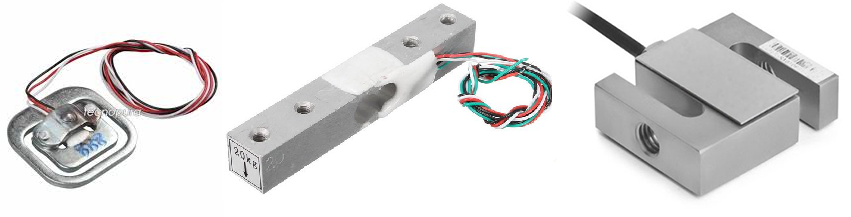
\includegraphics[scale=0.80]{img/celdas.png}
        \end{center}
	    \caption{Diferentes tipos de celdas de carga. \label{celdaspng}}
    \end{figure}

    Estos dispositivos requieren de un acondicionamiento de la señal analógica mediante un puente de ``Wheatstone'' y de un sistema mecánico que permita distribuir la fuerzas de manera proporcional sobre toda la superficie de contacto. Además, para entregar los datos de manera digital se requiere de una etapa de conversión por medio de un ADC.
    En cuestión de recursos económicos, tiempo y facilidad de uso, resulta más fácil utilizar una balanza digital comercial que fabricar una balanza desde cero. De esta forma se puede aprovechar el diseño mecánico y la ubicación del sensor y solo resta transformar la señal analógica a digital.
    
    En cuestión del prototipo, se utiliza el chip HX711 que incluye el puente de ``Wheatstone'' junto con una etapa de amplificación y el ADC simplificando significativamente la inclusión de circuitería.
    
    \begin{figure}[H]
	    \begin{center}
	    	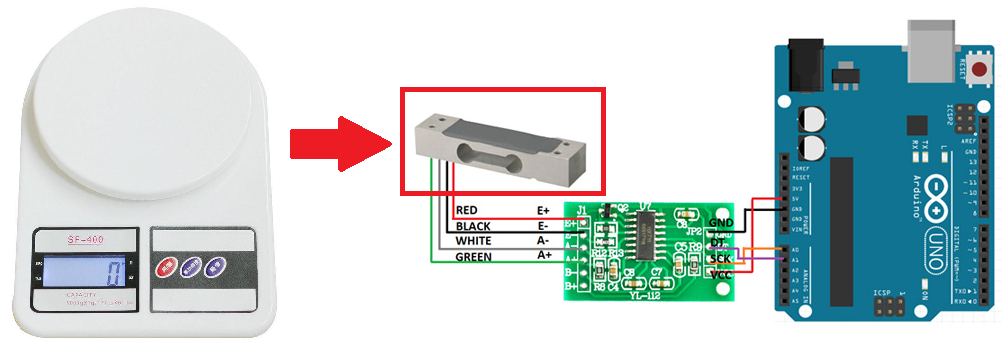
\includegraphics[scale=0.70]{img/pesaje.png}
        \end{center}
	    \caption{Medición general del peso. \label{pesajepng}}
    \end{figure}
    
    A modo general, el sistema electrónico encargado de pesar el alimento extraído del tanque y/o de adquirir el peso actual de un bovino (según corresponda) se observa en la Figura \ref{pesajepng}.
    % \textbf{CAMBIAR LA CELDA Y EL HX POR UN BLOQUE WHEATSTONE Y ADC}:

%%% Tek

% \subsubsection{TEMPORIZADOR}
% \subsubsection{Peso Balanza 2}
\subsubsection{Detección de alimento en el comedero}

Como se explicó en la Sección \ref{detectcomedero}, la detección de cantidad de alimento ingerido satisfactoriamente se logra si se cumplen 2 condiciones transitorias, ayudadas por un temporizador cuyo valor puede ser fijado por el productor ganadero. La detección de alimento se realiza mediante sensores infrarrojos ubicados en el costado vertical del comedero cuya distribución se puede apreciar en la Figura \ref{infra4png}.

\subsection{Actuadores}
\subsubsection{Motor de giro continuo}\label{mg995}

Como se mencionó antes, tanto el tornillo sin fin como las escobillas de barrido, son los elementos encargados de dosificar mecánicamente el alimento extraído desde la tolva y entregada en el comedero. No obstante, estos accesorios requieren de un dispositivo eléctrico para que puedan ejecutar su finalidad. Estos accesorios cumplen su papel mediante movimientos rotativos, realizados por motores DC de giro continuo.\\

Se considera pertinente dar prioridad a los servomotores que a otras modalidades, por su facilidad de uso, alimentación y manipulación mediante señales de control, reduciendo el uso de sistemas complejos como los requeridos para el uso de motores de alta potencia como los motores paso a paso.

Es importante recalcar el hecho que los motores deben estar en capacidad de garantizar un giro continuo para satisfacer el accionamiento mecánico del tornillo y de las escobillas de barrido, por lo que deben usarse motores especiales para $360^{o}$ de giro.
Por último, el motor debe estar en la capacidad de transmitir el torque necesario para girar su carga respectiva, por lo que en este caso, el motor debe contar adicionalmente con altas capacidades de torque.\\

En cuestión de prototipado de este proyecto, los servomotores de giro continuo usados son los $Tower Pro  MG995$ con una capacidad de torque a $5[V]$ de $9.4\left[\frac{kg}{cm}\right]$. Cuentan con engranaje metálico y pueden ser acoplados a otros accesorios externos mediante tornillos M3.

\begin{figure}[H]
    \begin{center}
    	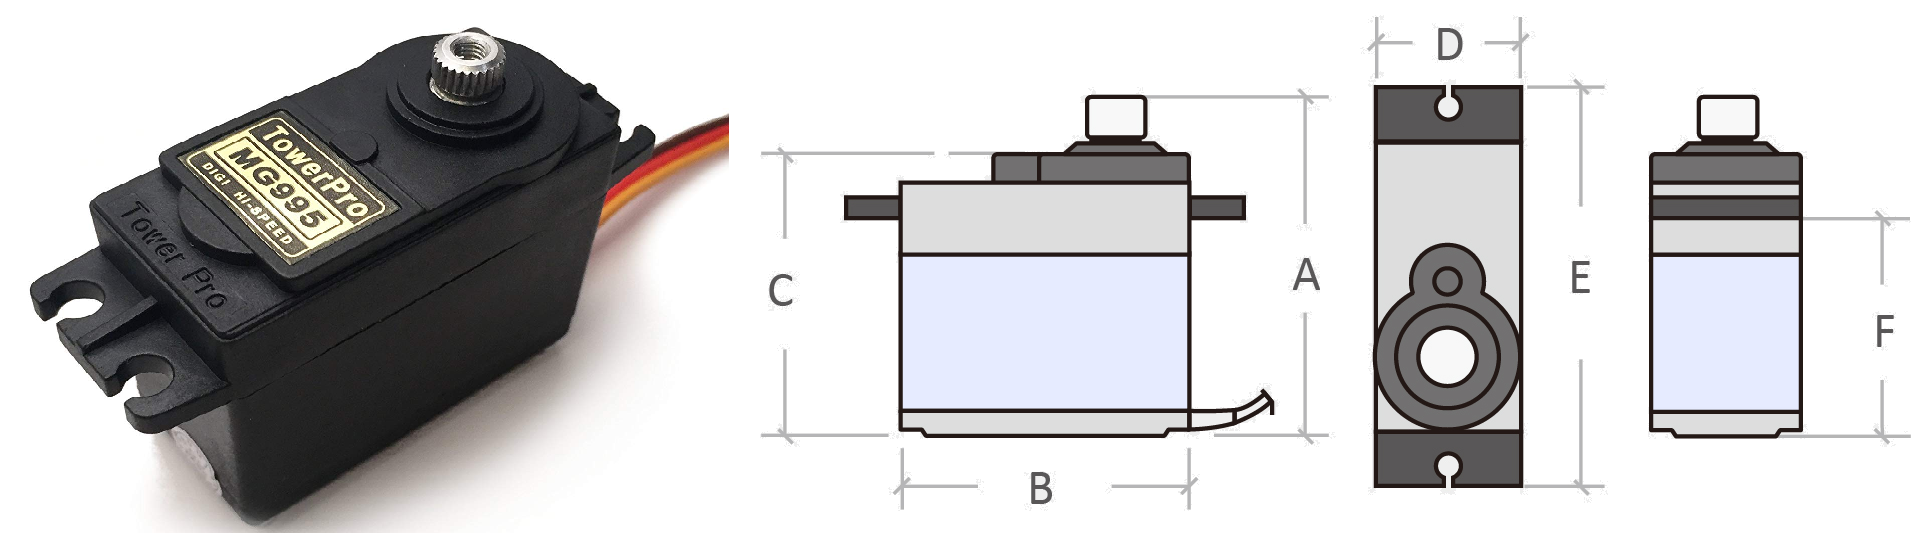
\includegraphics[scale=0.35]{img/servopro.png}
    \end{center}
    \caption{Servomotor de giro continuo TowerPro MG995. Tomada de \cite{servopro} \label{servopropng}}
\end{figure}

Donde $A=42.7[mm], B=40.9[mm], C=37[mm], D=20[mm], E=54[mm], F=26.8[mm]$.

\subsubsection{Sistema de Alarmas}

Aún cuando un sistema pueda ser diseñado con el objetivo de abarcar la mayoría de los posibles comportamientos, todo sistema está sujeto a posibles fallas o comportamientos indeseados. En este caso, para el desarrollo de este proyecto no se desean algunos comportamientos como los siguientes:

\begin{enumerate}
    \item Los bovinos ingieran su alimento de manera incorrecta,
    \item Se dé el caso que una res intente consumir más cantidad de alimento del especificado,
    \item Se agote el alimento a dosificar,
    \item Se ingresen animales no identificados,
    \item Entre otros.
\end{enumerate}

Para cuando se presenten estos casos indeseados se espera poder dar aviso al personal ganadero pertinente, por lo que se plantea el uso de diferentes alarmas como por ejemplo alarmas sonoras o alarmas visuales. Para el desarrollo del prototipo, se hará uso de alarmas visuales mediante un arreglo de diodos LED, y de alarmas sonoras mediante buzzers o pequeños altavoces.

\subsection{Microcontrolador}

Este proyecto está orientado al uso de dispositivos de manipulación de sensores y actuadores de bajo costo como los microcontroladores mencionados en el Capítulo \ref{cap4}. Estos serán los dispositivos encargados de recibir los datos sensados junto con los parámetros de entrada entregados por el productor ganadero (Usuario). También están encargados de procesar los datos y hacer la activación de los actuadores respectivos según sea el caso. Finalmente realizan el registro de los datos correspondientes en la(s) base(s) de datos. Como posibilidad adicional pueden ser conectados a dispositivos de representación gráfica o a interfaces gráficas de usuario (GUI) (\textit{\textbf{No incluidas dentro de los alcances de este proyecto}})

En este proyecto, se utiliza un Arduino Mega. Este microprocesador facilita la prueba del prototipo debido a su gran variedad de pines analógicos y digitales con lo que se puede lograr una conexión completa de los dispositivos a utilizar sin la necesidad de módulos externos o módulos adicionales.

% \pagebreak
% \subsubsection{Arduino}

% \subsection{MicroProcesador}
% \subsubsection{Arduino}

%  \item \textbf{Pesaje de porción: }
    
%     En lo que respecta al pesaje de la porción de alimento se ha preestablecido que ésta sería pesada a medida es extraída del tanque de almacenamiento para corroborar la cantidad ($en gramos$) que se entregará al bovino correspondiente. Para ello se requiere de una herramienta que permita medir peso. Los sensores especializados para este tipo de mediciones son las galgas extensométricas o las celdas de carga 
